\chapter{Propuesta de Solución}\label{chapter: proposedsolution}

En el presente capítulo se abordará la metodología seguida para diseñar el experimento propuesto en este trabajo \ref{experiment_defref}. Primeramente, se expondrá un marco teórico que formaliza la definición del problema a tratar, esto con el objetivo de presentar los conocimientos base tenidos en cuenta para los enfoques probados. Luego, se detallan los primeros acercamientos desechados \ref{approaches_considered}, argumentando las deficiencias de estos a la hora de arrojar resultados consistentes para la tarea que se desea desarrollar. Finalmente, se detalla la metodología definitiva a implementar, teniendo en cuenta la experiencia obtenida de las anteriores y mostrando su robustez para el análisis experimental \cite{}.

De forma general, el componente común para cada vía de solución constituye la presencia de un Gran Modelo de Lenguaje, pues representan los modelos más recientes utilizados para la tarea en cuestión; además, ofrecen resultados alentadores para el caso de traducción a lenguaje \textit{SQL} según lo visto en la sección \ref{llm_approach}. Por lo tanto, tiene sentido probar su eficacia para traducir a código en \textit{Cypher}, ya que ambos presentan similitudes como lenguajes formales declarativos para consultar bases de datos. Dicho modelo será analizado como una ``caja negra'' capaz de hacer tareas de traducción de lenguaje natural a una consulta semánticamente equivalente en el lenguaje \textit{Cypher}.

Para cada vía de solución se deberá considerar el despliegue de un sistema de gestión de bases de datos para alguna BDOG, ya que es en este componente donde se almacenará la información a extraer por consultas en un lenguaje orientado a este tipo de almacenamiento. En el caso particular de este trabajo, se considerará el uso de \textit{Neo4J}, con el cual se puede interactuar a partir del lenguaje \textit{Cypher} ya mencionado. Por esto, es importante considerar la implementación de un módulo intermedio para interactuar con una instancia del sistema de gestión \textit{Neo4J}.

El enfoque de \textit{prompt engineering} a utilizar será ZSL, por lo tanto, los textos de entrada que se le darán al modelo para la generación de código \textit{Cypher} no contendrán ejemplos de pares de lenguaje natural con su correspondiente traducción al lenguaje de consulta objetivo. Por lo tanto, se tomarán algunas ideas experimentadas en el estado del arte para \textit{SQL} vistas en la sección \ref{}.

\subsection{Definición del problema \textit{Text-to-Cypher}} \label{problem_definition}
Dentro del ámbito de las bases de datos y las consultas que las acceden, existe una tarea particularmente compleja: traducir preguntas formuladas en lenguaje natural a un lenguaje de consulta estructurado como \textit{Cypher}. Dada una pregunta $Q$, formulada en lenguaje cotidiano, y un esquema de base de datos $S$, el cual se compone a partir del tuplo ${N, A, R}$, donde encontramos múltiples nodos $N$ (que representan instancias de una entidad en la base de datos), atributos $C$ (tanto en nodos como en relaciones) y relaciones entre pares de nodos $R$. La problemática subyacente en el proceso de convertir \textit{Text-to-Cypher} se centra en generar una consulta en lenguaje \textit{Cypher} $Y$ que sea equivalente y responda adecuadamente a la pregunta inicial $Q$ realizada por un usuario humano.

\subsection{LLM para resolver \textit{Text-to-Cypher}} \label{llmfortext2cypher}

Con el auge de la inteligencia artificial y el aprendizaje automático, la tarea de convertir texto en lenguaje natural a código en \textit{Cypher} ha sido recientemente abordada a través de técnicas modernas. En trabajos más recientes, algunos investigadores, \cite{sunetal2023} \cite{liuetal2023}, han abogado por formular esta tarea como un desafío de generación. Utilizando lo que se conoce como "\textit{prompts}" o indicaciones $P$, es posible dirigir y guiar a un gran modelo de lenguaje $M$ en esta labor. Este modelo, una vez entrenado, puede estimar una distribución de probabilidad sobre posibles consultas \textit{Cypher} $Y$. De esta forma, el modelo es capaz de generar, paso a paso y token por token, una consulta apropiada.

La fórmula subyacente para generar la consulta $Y$ se estructura como:
$$P_M(Y|P, S, Q) = \prod_{i=1}^{|Y|}{P_M(Y_i | P, S, Q, Y < i)}$$ \label{llm_query_generation}

Para simplificar, $Y< i$ se refiere al fragmento inicial o prefijo de la consulta \textit{Cypher} que se está construyendo. Mientras que $P_M(Yi|*)$ denota la probabilidad condicional asociada con la generación del i-ésimo token, considerando factores como el prefijo existente $Y<i$, la indicación $P$, el esquema $S$ y la pregunta original $Q$.

Uno de los hallazgos más reveladores en el campo reciente es el concepto de aprendizaje en contexto (ICL, por sus siglas en inglés) \cite{icldefinition}, en el cual, grandes modelos de lenguaje pueden adaptarse y aprender de unos pocos ejemplos presentados en un contexto específico. Esta estrategia, defendida por varios investigadores \cite{sunetal2023} \cite{minetal2022} \cite{pourrezandrafiei2023}, ha mostrado que los LLMs pueden abordar y dominar una amplia variedad de tareas complejas con una cantidad limitada de datos. Sin embargo, hay un equilibrio que mantener: agregar más ejemplos conlleva un aumento en los costos, tanto en términos de mano de obra para preparar esos ejemplos como en términos de costos de procesamiento y tokens al interactuar con APIs avanzadas como la de OpenAI \cite{openaiapi}. En este estudio, el foco recae en trabajar eficientemente con indicaciones al modelo de lenguaje sin requerir ejemplos adicionales.

\section{Propuesta de solución diseñada} \label{designed_proposal}

En el desarrollo de sistemas de bases de datos, la interacción eficiente y la gestión de esquemas son fundamentales para la manipulación y el mantenimiento de datos. En este contexto, se ha desarrollado una arquitectura de software compuesta por varios componentes interconectados diseñados para interactuar con una base de datos de grafos, con especial atención en \textit{Neo4J}, un sistema de manejo de bases de datos basado en grafos.

Uno de los componentes clave de esta arquitectura es el \texttt{GraphContractor}, un módulo diseñado para facilitar la interacción con la base de datos. Este componente actúa como intermediario entre la aplicación y la base de datos, manejando la lógica necesaria para establecer conexiones, ejecutar consultas y manejar los resultados. La modularidad del \texttt{GraphContractor} permite su reutilización y fácil mantenimiento, además de proporcionar una capa de abstracción que simplifica las operaciones de la base de datos para los desarrolladores.

Para la generación de esquemas de la base de datos, se ha creado el \texttt{SchemaMaker}, una herramienta automatizada que se encarga de construir los esquemas necesarios para \textit{Neo4J}. Esta herramienta juega un rol crucial en la estructuración de la base de datos, ya que define la organización de nodos, relaciones, propiedades y restricciones. El \texttt{SchemaMaker} garantiza que la base de datos esté correctamente configurada para cumplir con los requisitos del dominio y las necesidades de la aplicación, asegurando así la integridad y coherencia de los datos.

En la interfaz entre el lenguaje natural y la base de datos, se ha integrado el modelo de lenguaje \texttt{GPT-4}, utilizado como una ''caja negra'' para la traducción de consultas en lenguaje natural a \textit{Cypher}, el lenguaje de consulta para \textit{Neo4J}. La capacidad de \texttt{GPT-4} para comprender y generar texto hace posible que los usuarios realicen consultas complejas sin necesidad de conocer la sintaxis específica de \textit{Cypher}. Para mejorar la precisión y relevancia de las traducciones, se ha elaborado una plantilla de prompt que se nutre de la salida del \texttt{SchemaMaker}. Esta plantilla guía al modelo de lenguaje proporcionando contexto y estructura, lo que permite que \texttt{GPT-4} genere consultas \textit{Cypher} más precisas y eficientes.

Finalmente, se ha desarrollado el \texttt{DBSeeder}, un componente encargado de poblar la base de datos de \textit{Neo4J} con datos iniciales o de prueba. Utilizando consultas Cypher generadas por el modelo de lenguaje \texttt{GPT-4}, el DBSeeder trabaja en conjunto con el GraphContractor para insertar nodos, atributos y relaciones en la base de datos. Esta funcionalidad es especialmente valiosa en las etapas de desarrollo y prueba, donde se requiere de una base de datos poblada para validar el diseño y la lógica de la aplicación. Además, el DBSeeder está diseñado para operar dentro de un contenedor de Docker, lo que ofrece ventajas significativas en términos de portabilidad, escalabilidad y aislamiento del entorno de desarrollo.

Cada uno de estos componentes representa un eslabón en la cadena de herramientas que permitirán interactuar con la base de datos de grafos de manera más intuitiva y automatizada. La integración de tecnologías avanzadas como \texttt{GPT-4} en el proceso no solo mejora la accesibilidad para los usuarios finales sino que también agiliza el ciclo de desarrollo, ofreciendo un enfoque moderno y eficiente en la gestión de bases de datos de grafos como \textit{Neo4J}.

\subsection{Interacción con una base de datos \textit{Neo4J}} \label{graph_contractor}

El componente \texttt{GraphContractor} actúa como un facilitador o intermediario entre el usuario y la base de datos \textit{Neo4J}. Su propósito es simplificar las tareas de conexión y ejecución de consultas contra la base de datos, manejando internamente los detalles de la comunicación y posibles excepciones.

Al instanciar \texttt{GraphContractor}, se le proporciona una URL, junto con un nombre de usuario y contraseña para la autenticación. Luego, esta herramienta intenta establecer una conexión con la instancia de la base de datos \textit{Neo4J} en la URL especificada. Si la conexión es exitosa, el \texttt{GraphContractor} estará listo para ejecutar consultas. Si la conexión falla, por ejemplo, debido a problemas con la red o las credenciales de acceso, se informará al usuario al respecto con un mensaje informativo.

Una vez que el \texttt{GraphContractor} está conectado a la base de datos, es posible realizar consultas a una base de datos objetivo. Para dicha tarea, este acepta una cadena de texto que representa la consulta \textit{Cypher} a ejecutar. Al efectuar dicha funcionalidad con una consulta de \textit{Cypher} válida, \texttt{GraphContractor} la ejecutará en la base de datos y devolverá los resultados. Si ocurre algún error durante la ejecución de la consulta, como una sintaxis incorrecta de \textit{Cypher} o un problema de conexión, el error se capturará y se presentará al usuario, ofreciendo retroalimentación inmediata.

\begin{figure}[H]\label{gcimage}
	\centering
	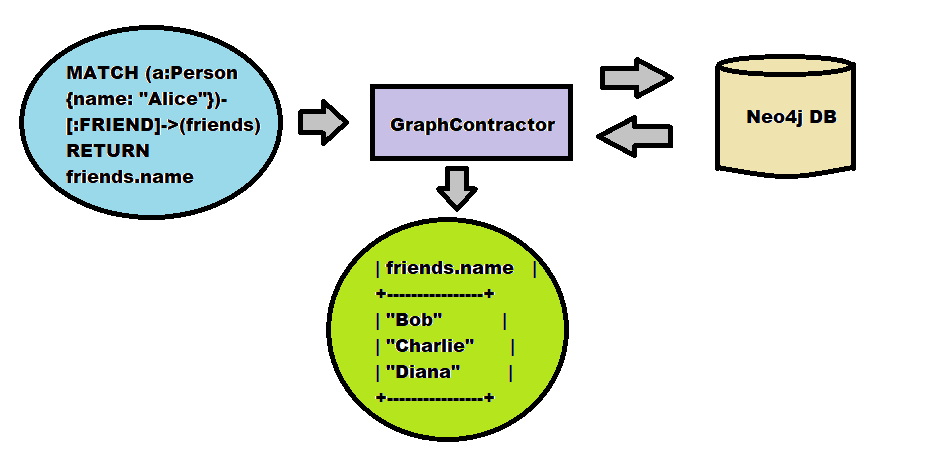
\includegraphics[width = 0.9\textwidth]{./Graphics/graph_contractor}
	\caption{Flujo de funcionamiento del componente \texttt{GraphContractor}.}
\end{figure}

En resumen, \texttt{GraphContractor} encapsula la complejidad de la gestión de la conexión a la base de datos y la ejecución de consultas, proporcionando una interfaz simplificada para interactuar con \textit{Neo4J}. Esto permite a los usuarios centrarse en la lógica de sus consultas y manejo de datos, en lugar de en los detalles subyacentes de la implementación de la base de datos.

\subsection{Almacenamiento de información en una base de datos \textit{Neo4J}} \label{dbseeding}

El componente \texttt{DBSeeder} es una herramienta diseñada para cargar datos en una base de datos de grafos. Su propósito es automatizar el proceso de toma de datos estructurados y su inserción en la base de datos, creando nodos y relaciones entre ellos según se define en los datos de entrada.

Al inicializar esta herramienta, se le proporcionan dos piezas de información esenciales: un conjunto de conocimientos que describe la estructura de la base de datos y una ruta a un archivo que contiene los datos a ser sembrados en la base de datos. Estos datos de entrada son esenciales para guiar el proceso de sembrado.

Una vez configurada, la herramienta tiene la capacidad de procesar los datos de entrada. Esto se realiza leyendo cada línea del archivo de datos, donde cada línea representa un conjunto de información que debe ser transformada en elementos dentro de la base de datos. La herramienta analiza cada línea para comprender y aislar las partes que corresponden a entidades y las relaciones entre ellas.

Para cada conjunto de datos, la herramienta verifica si los elementos ya existen en la base de datos. Si no es así, procede a crear nuevos nodos que representan entidades y luego establece relaciones entre estos nodos, basándose en la relación especificada en los datos.

\begin{figure}[H]\label{dbseeder}
	\centering
	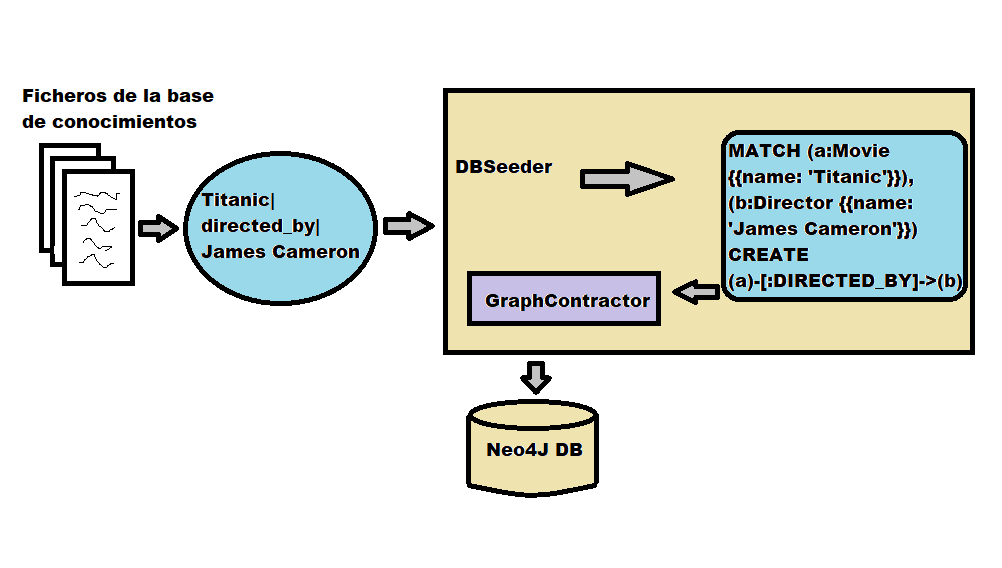
\includegraphics[width = 0.9\textwidth]{./Graphics/dbseeder}
	\caption{Flujo de funcionamiento del componente \texttt{DBSeeder}.}
\end{figure}

El proceso de llenado en la base de datos asegura que no se introduzcan duplicados y que los datos se estructuren correctamente esta la base de datos de acuerdo con sus reglas y definiciones. Al finalizar, la base de datos debería reflejar una red de nodos interconectados que representan tanto las entidades como las relaciones definidas en el archivo de datos original. Este proceso es fundamental para preparar la base de datos para su uso en aplicaciones que requieren acceso a datos relacionales y estructurados en forma de grafo.

\subsection{Selección del modelo} \label{model_selection}

La selección de \texttt{GPT-4} para la generación de código a partir de lenguaje natural utilizando aprendizaje \textit{Zero-Shot} (ZSL) está justificada por varias razones fundamentadas en investigaciones y comparaciones técnicas recientes.  \texttt{GPT-4} es un avance significativo respecto a sus predecesores, construido sobre la arquitectura de  \texttt{GPT-3} pero alcanzando nuevos niveles de rendimiento y escala \cite{}. Este modelo mejora en la corrección factual de las respuestas y reduce las "alucinaciones", donde el modelo comete errores de hecho o razonamiento, obteniendo un $40\%$ más de precisión que  \texttt{GPT-3.5} en las pruebas de rendimiento factual internas de OpenAI \cite{}.

El modelo  \texttt{GPT-4} se basa en la arquitectura Transformer, que utiliza mecanismos de atención para procesar texto, y se ha mejorado con una mezcla de expertos (MoE) para lograr un modelo con aproximadamente $1.76$ billones de parámetros, un orden de magnitud mayor que  \texttt{GPT-3} \cite{}. Además, estudios recientes han mostrado que  \texttt{GPT-4} supera a  \texttt{GPT-3.5} en aprendizaje zero-shot en casi todas las tareas evaluadas, lo que incluye una variedad de dominios de razonamiento como deductivo, inductivo, abductivo, analógico, causal y multi-salto, a través de tareas de preguntas y respuestas \cite{}.

Además, el modelo  \texttt{GPT-4} emplea técnicas de \textit{fine-tuning} y Aprendizaje por Refuerzo con Retroalimentación Humana (RLHF), lo que le permite ser un modelo multimodal robusto capaz de procesar entradas textuales y visuales y generar salidas basadas en texto \cite{}. Este enfoque ha demostrado ser eficaz en la mejora de las capacidades de razonamiento de los modelos de lenguaje grandes (LLMs), lo que lo hace especialmente adecuado para tareas complejas que requieren razonamiento, como la traducción de lenguaje natural a lenguaje de consulta formal \cite{}.

\begin{table}[H]
  \centering
  \caption{Rendimiento de GPT-4 en referencias académicas. \cite{}}
  \begin{tabularx}{\textwidth}{Xcccc}
    \toprule
    & \textbf{GPT-4} & \textbf{GPT-3.5} & \textbf{LM SOTA} & \textbf{SOTA} \\
    \midrule
    \textbf{MMLU} & 86.4\% & 70.0\% & 70.7\% & 75.2\% \\
    \textbf{HellaSwag} & 95.3\% & 85.5\% & 84.2\% & 85.6\% \\
    \textbf{AI2 Reasoning Challenge (ARC)} & 96.3\% & 85.2\% & 85.2\% & 86.5\% \\
    \textbf{WinoGrande} & 87.5\% & 81.6\% & 85.1\% & 85.1\% \\
    \textbf{HumanEval} & 67.0\% & 48.1\% & 26.2\% & 65.8\% \\
    \textbf{DROP} & 80.9\% & 64.1\% & 70.8\% & 88.4\% \\
    \textbf{GSM-8K} & 92.0\% & 57.1\% & 58.8\% & 87.3\% \\
    \bottomrule
  \end{tabularx}
  \label{tab:my_label}
\end{table}

En comparación con otros modelos como \texttt{PALM, Chinchilla, LaMDA, LLaMA} y \texttt{Gopher}, que también han evaluado sus habilidades de razonamiento,  \texttt{GPT-4} se destaca por su capacidad mejorada de aprendizaje zero-shot y por el uso de estrategias de prompting refinadas para mejorar aún más su rendimiento en tareas de razonamiento, lo que lo convierte en una elección prometedora para la generación de código \cite{}.

\begin{figure}[H]\label{simplegpt4}
	\centering
	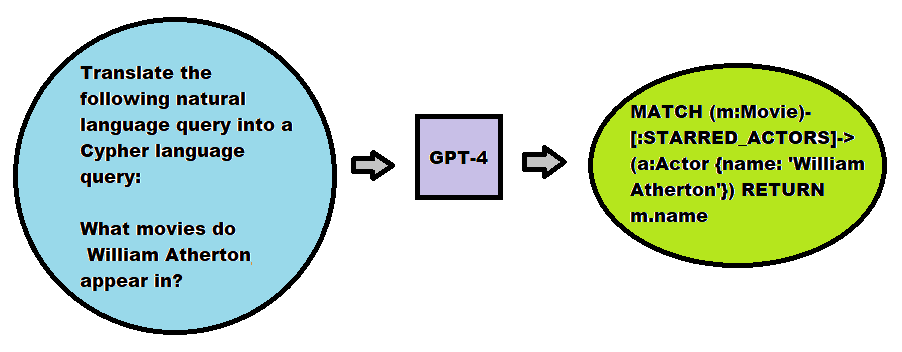
\includegraphics[width = 0.9\textwidth]{./Graphics/simplegpt4use}
	\caption{Ejemplo básico sobré como utilizar \texttt{GPT-4} para traducir lenguaje natural en lenguaje de consulta \textit{Cypher}.}
\end{figure}

\subsection{Diseño de la información entrada al LLM} \label{prompt_design}

Tal y como se mostró en la sección anterior, el uso de \texttt{GPT-4} para la tarea de traducción no resulta complicado, pues este es utilizado como una gran ``caja negra'' capaz de realizar operaciones que se le indiquen en un texto (\textit{prompt}) de entrada. Debido a esto, también es importante mencionar que no cualquier entrada es efectiva o suficiente para obtener el resultado esperado \cite{promtpengineeringeffectiveness}. Al proceso de diseñar una entrada de calidad para que el modelo realice una tarea específica exitosamente se denomida \textit{prompt engineering} \cite{promptengineering}. 

Dado que la hipótesis central de este trabajo se basa en el uso del aprendizaje \textit{Zero-Shot} (ZSL), el texto de entrada al modelo \texttt{GPT-4} no puede contener ejemplos de cómo traducir una consulta en lenguaje humano a lenguaje \textit{Cypher}, es decir, no deberá reflejar contenido demostrativo de la tarea a realizar, lo cual se justifica por la misma definición del enfoque ZSL \ref{zeroshotlearning}. Además, como parte de la información de entrada al modelo para este tipo de tareas, es común añadir una descripción de la estructura de la base de datos a consultar \cite{samplepromptsnl2ql1} \cite{samplepromptsnl2ql2}, lo cual se conoce como esquema de la base de datos \cite{dbschema}. 

Por lo mencionado anteriormente, el texto de entrada al modelo deberá contener:

\begin{itemize}
	\item \textbf{La tarea a ejecutar}: Se le describirá al modelo la tarea a realizar, mencionando los datos que recibirá de entrada y el formato en que se desea obtener la respuesta.
	\item \textbf{Esquema de la base de datos}: Se especificará el contenido de la base de datos objetivo en forma de grafo, mencionando las entidades, relaciones y atributos presentes en la misma.
	\item \textbf{Consulta en lenguaje natural}: En este caso, se añadirá la consulta en lenguaje natural humano a traducir.
\end{itemize}

Para la obtención del esquema de la base de datos de tipo \textit{Neo4J} se diseñó el componente \texttt{SchemaMaker}. Con el fin de elaborar la descripción de la estructura de la fuente de datos objetivo, este recibe los nombres de las entidades, las relaciones y los atributos presentes en la misma. Dicha información la obtiene auxiliándose del componente \texttt{GraphContractor} \ref{graph_contractor}, mediante el cual se realizan las consultas en lenguaje \textit{Cypher} pertinentes a la instancia de la fuente de datos \textit{Neo4J} en cuestión. A continuación se muestra un ejemplo del funcionamiento de la herramienta \texttt{SchemaMaker}:

\subsection{Caso de estudio} \label{sample_case}